\subsection{Reciprocal behavior of electric and magnetic fields}

\begin{frame}{Reciprocal behavior of electric and magnetic fields}
    \begin{columns}
        \column{0.5\textwidth}
        \vspace{-7mm}
        \begin{center}
            \textcolor{BlueDefault}{Faraday's law}
        \end{center}
        
        \begin{itemize}
            \item \( \nabla \times \mathbf{E} = - \dfrac{\partial \mathbf{B}}{\partial t} \).
            \item \( \mathcal{E} = - \dfrac{ \mathrm{d} \Phi }{ \mathrm{d} t }\).
            \item Motional emf \& Faraday emf. \cite{Griffiths_2023}
        \end{itemize}

        \begin{figure}[!htb]
        \centering
        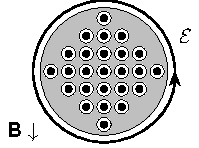
\includegraphics[width=0.6\textwidth]{Figures/Faraday_law.pdf}
        \caption{Faraday's law.}
        \label{Faraday_law}
        \end{figure}

        \column{0.5\textwidth}
        \vspace{-7mm}

        \begin{center}
            \textcolor{BlueDefault}{Ampere's law}
        \end{center}
        
        \begin{itemize}
            \item \( \nabla \times \mathbf{H} = \mathbf{j} + \dfrac{\partial \mathbf{D}}{\partial \mathbf{t}} \).
            \item Displacement current \( \mathbf{j}_D \equiv \dfrac{\partial \mathbf{D}}{\partial \mathbf{t}} \).
        \end{itemize}
        \vspace{-1mm}
        \begin{figure}[!htb]
        \centering
        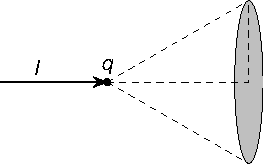
\includegraphics[width=0.8\textwidth]{Figures/Displacement_current.pdf}
        \caption{Displacement current.\cite{Purcell_Morin_2013}}
        \label{Displacement_current}
        \end{figure}
    \end{columns}
\end{frame}